% last updated in April 2002 by Antje Endemann
% Based on CVPR 07 and LNCS, with modifications by DAF, AZ and elle, 2008 and AA, 2010, and CC, 2011; TT, 2014

\documentclass[runningheads]{llncs}
\usepackage{float}
\usepackage{graphicx,subcaption}
\usepackage{amsmath,amssymb} % define this before the line numbering.
\usepackage{ruler}
%\usepackage{color}
\usepackage[usenames, dvipsnames]{color}
\graphicspath{ {figures/} }
\usepackage[width=122mm,left=12mm,paperwidth=146mm,height=193mm,top=12mm,paperheight=217mm]{geometry}
\usepackage[breaklinks=true,bookmarks=false]{hyperref}
\setlength{\intextsep}{10pt plus 2pt minus 2pt}


%%%%%%%%%%%%%%COLOR MACROS FOR EACH EDITOR%%%%%%%%%%%%%
\newcommand{\Leon}[1]{{\color{BurntOrange}{#1}}}
\newcommand{\Arik}[1]{{\color{LimeGreen}{#1}}}
\newcommand{\Guy} [1]{{\color{RoyalBlue}{#1}}}
\newcommand{\RevComment} [1]{{\color{Red}{#1}}}
%%%%%%%%%%%%%%OTHER MACROS%%%%%%%%%%%%%
\newcommand*{\eg}{{\em e.g.}\@\xspace}
\newcommand*{\ie}{{\em i.e.}\@\xspace}
\newcommand*{\etal}{{\em et al.}\@\xspace}

\begin{document}
% \renewcommand\thelinenumber{\color[rgb]{0.2,0.5,0.8}\normalfont\sffamily\scriptsize\arabic{linenumber}\color[rgb]{0,0,0}}
% \renewcommand\makeLineNumber {\hss\thelinenumber\ \hspace{6mm} \rlap{\hskip\textwidth\ \hspace{6.5mm}\thelinenumber}}
% \linenumbers
\pagestyle{headings}
\mainmatter
\def\ECCVSubNumber{1411}  % Insert your submission number here

\title{Supplemental Material} % Replace with your title

\titlerunning{ECCV-16 submission ID \ECCVSubNumber}

\authorrunning{ECCV-16 submission ID \ECCVSubNumber}

\author{Anonymous?}
\institute{Paper ID \ECCVSubNumber}


\maketitle

\section{Performance as function of training composites}
We observe performance of our method when training with different portions of the data. We report results when learning on 10\%, 30\% and 50\% of the composites, as shown in Figure~\ref{fig:learning_portions}. We further verify result consistency by pruning composites with less training examples than a certain threshold. We plot performance as a function of this threshold. In the Scene-Attribute classification experiment (left set of 3 plots) we achieve results comparable to cross validation performance using as little as 10\% of the composites; training with bigger portion of the data led to little further improvements. In the Object-Attribute detection experiment (right set of 3 plots) we achieve close to cross-validation performance when using 30\% of the composites to train our regressor. A similar trend is observed in the Object-Relationship experiment (not shown).



\begin{figure}
    \centering
    \subfloat{{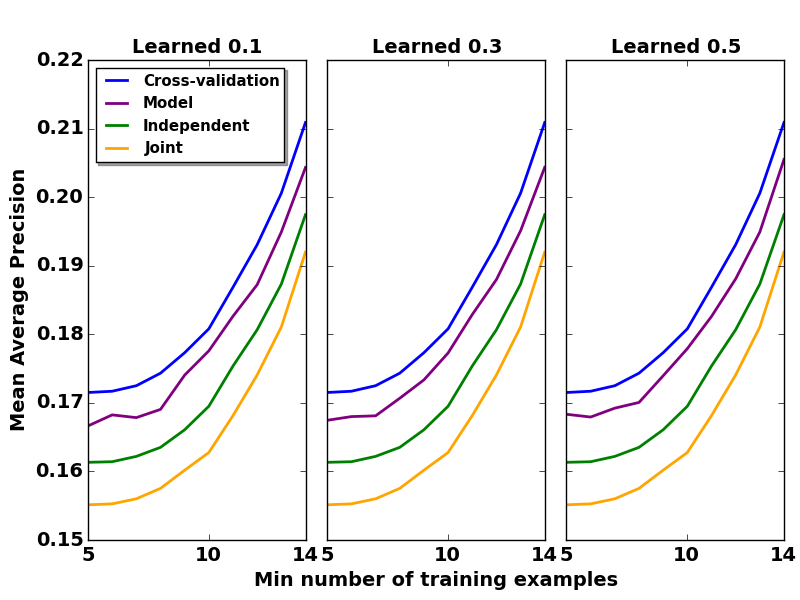
\includegraphics[width=5cm]{att_scene_multiple_partitions.png} }}%
    \qquad
    \subfloat{{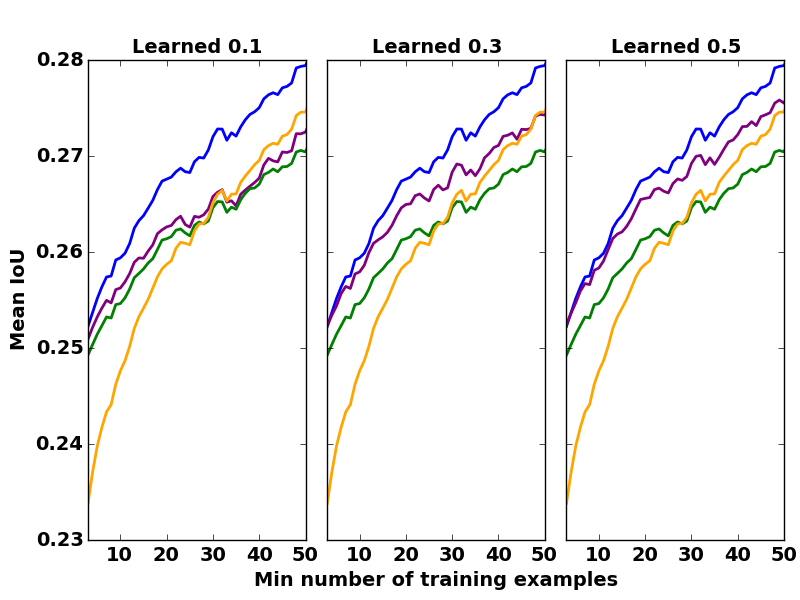
\includegraphics[width=5cm]{obj_att_multiple_partitions.png} }}%
    \caption{{\bf Performance for different fraction of composites used for learning:} Illustrated  are scene-attribute performance on SUN  (left) and object-attribute perfromance for SceneGraph dataset (right). Our model approaches cross-validation performance with only a fraction (0.1) or 10\% of scene-attribute and (0.3) or 30\% of object-attribute composites.}%
    \label{fig:learning_portions}%
    \vspace{-0.2in}
\end{figure}


\section{Learned weights}
The assumption that each dataset may contain unique patterns for optimal strategy selection stands at the core of our approach. However, that said, we have observed somewhat similar trends in learned weights for different experiments and datasets, as is demonstrated in Figure~\ref{fig:learned_weights}. For example, large median value of pairwise distance ($\mathbf{f_4}$) tends to lead to joint strategy selection, whereas large mean pairwise distance ($\mathbf{f_5}$) has the opposite effect. Some intuition for this trend is given on the rightmost plot, showing the effect of the above feature values on our selection. Also note that for each composite we concatenate features collected from different composite parts to obtain our vector representation.

\section{SceneGraph retrieval qualitative results}
We also visualize additional examples for SceneGraph retrieval. We visualize object localization performance by plotting grounded object locations, obtained using CRF inference (see main paper for description) and comparing to ground truth annotations. We use graphs where each object is trained fully independently, fully jointly, or partly jointly (when the joint configuration is selected by our model prediction). Effective selection of joint object configuration (object+attribute, object+relationship) made by our model provides more accurate detectors. These detectors in turn output better confidence scores used as the unary terms in the CRF inference, leading to a better solution overall, as visualized in Figure~\ref{fig:scene_graph_retrieval}. 


\begin{figure}[t]
    \centering
    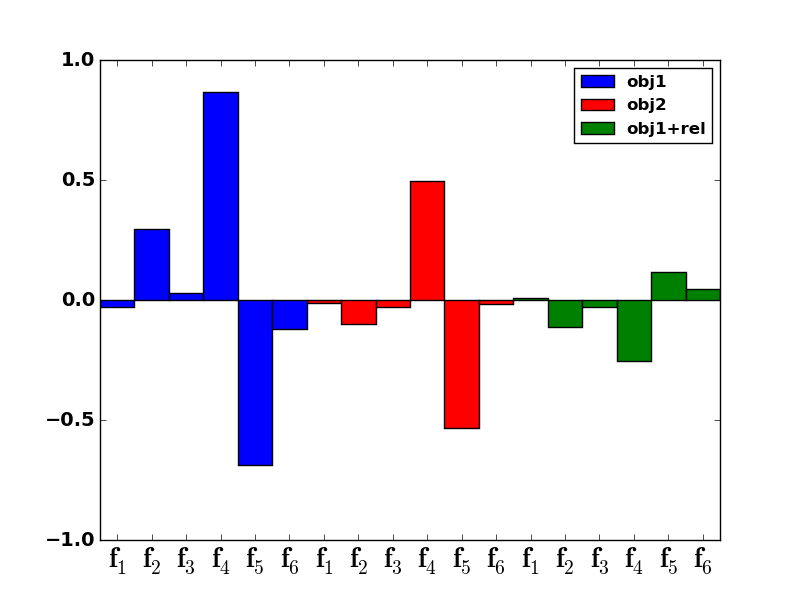
\includegraphics[width=3.7cm]{obj_rel_o1r_o2_coeffs.png}\hspace{0em}
    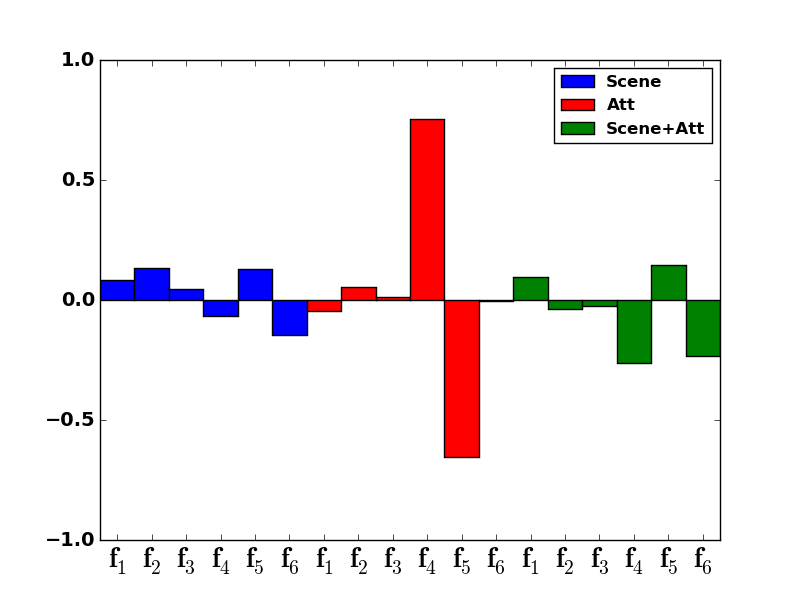
\includegraphics[width=3.7cm]{att_scene_coeffs.png}\hspace{0em}
    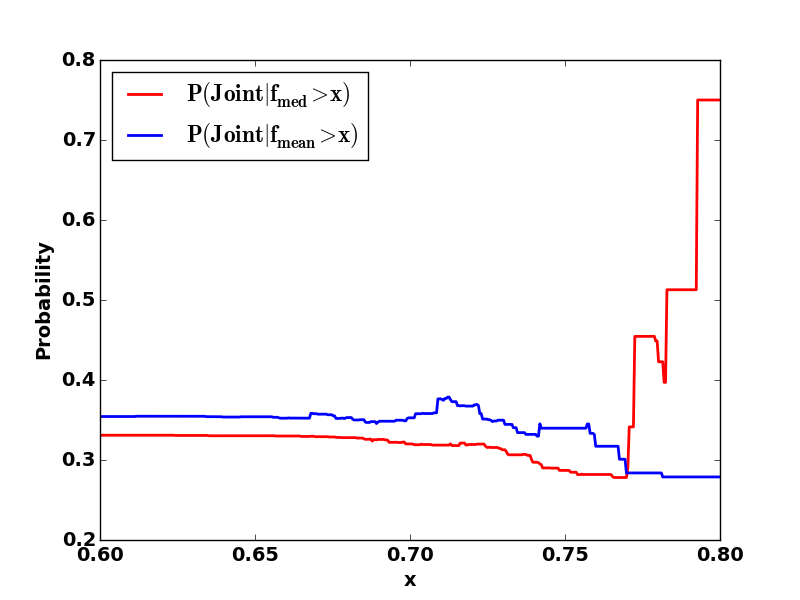
\includegraphics[width=3.7cm]{att_scene_prob_joint_given_med_mean.png}
    \caption{{\bf Illustration of learned feature weights:} Weights corresponding to Object-Relationship and Scene-Attribute are illustrated in (left) and (middle). Probability of joint selection given certain features size is shown on (right).}%
    \label{fig:learned_weights}
    % \RevComment{Ablation experiments that show the importance of the features in fs would be useful. It would be interesting to see which of the features are non-zero if you use an L1 penalty on w in Eq 6}
\end{figure}


\begin{figure}[H]
    \centering
%    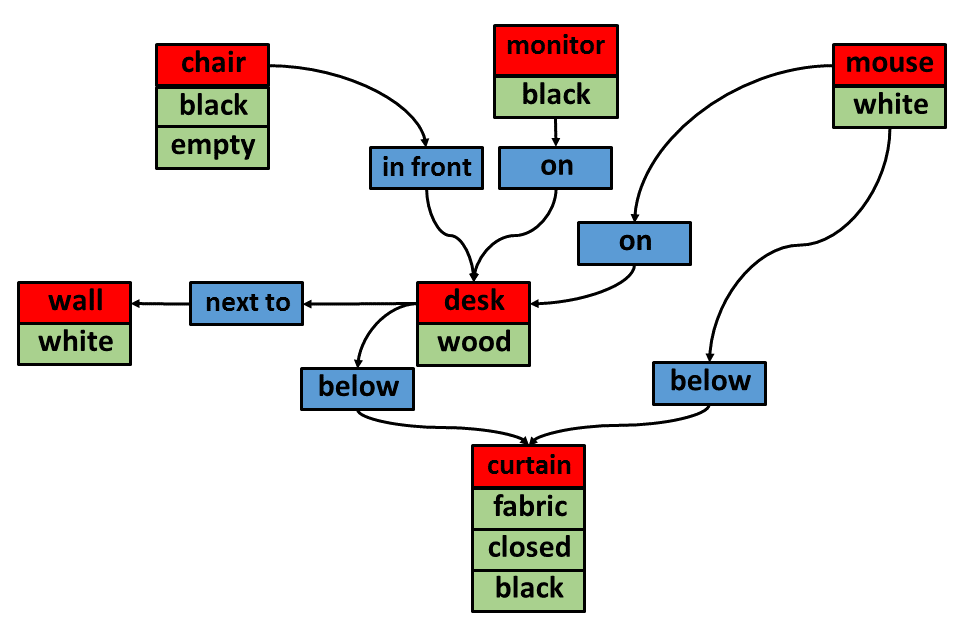
\includegraphics[width=2.7cm]{3_scene_graph.png}\hspace{0em}
%    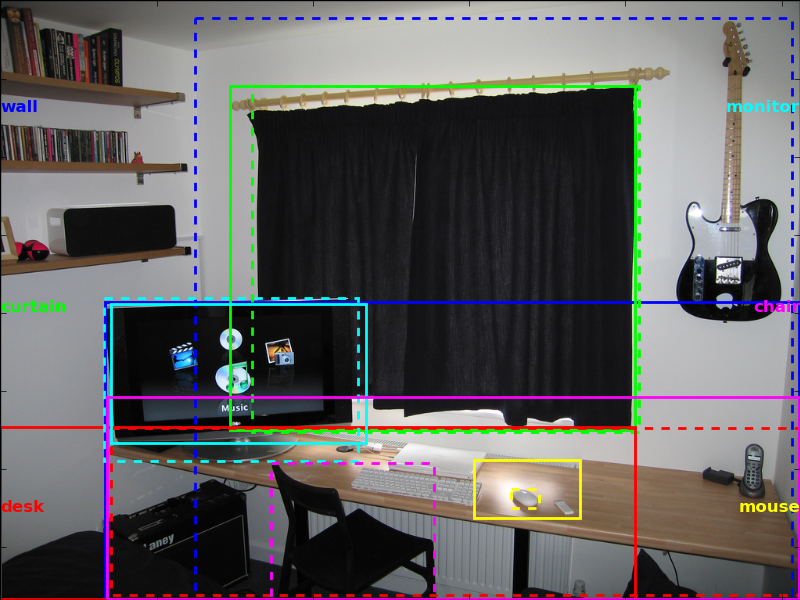
\includegraphics[width=2.7cm]{3_ind.png}\hspace{0em}
%    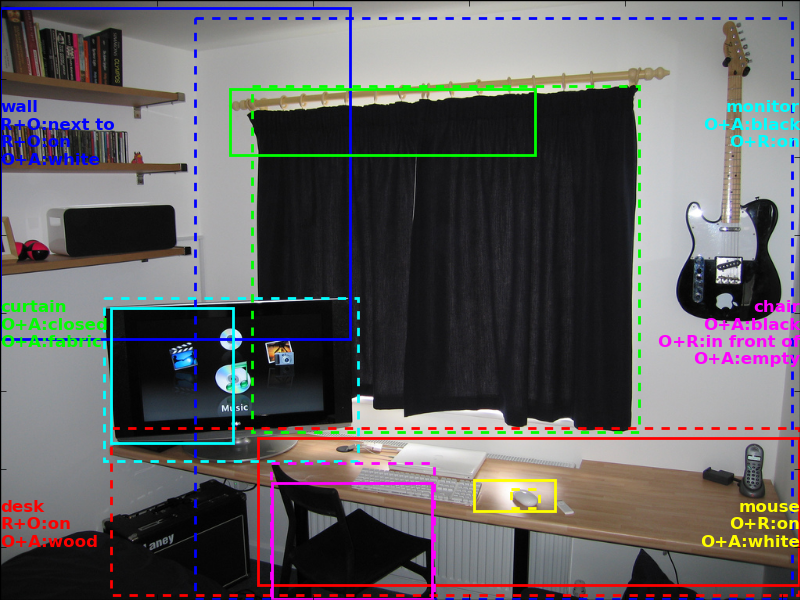
\includegraphics[width=2.7cm]{3_joint.png}\hspace{0em} 
%    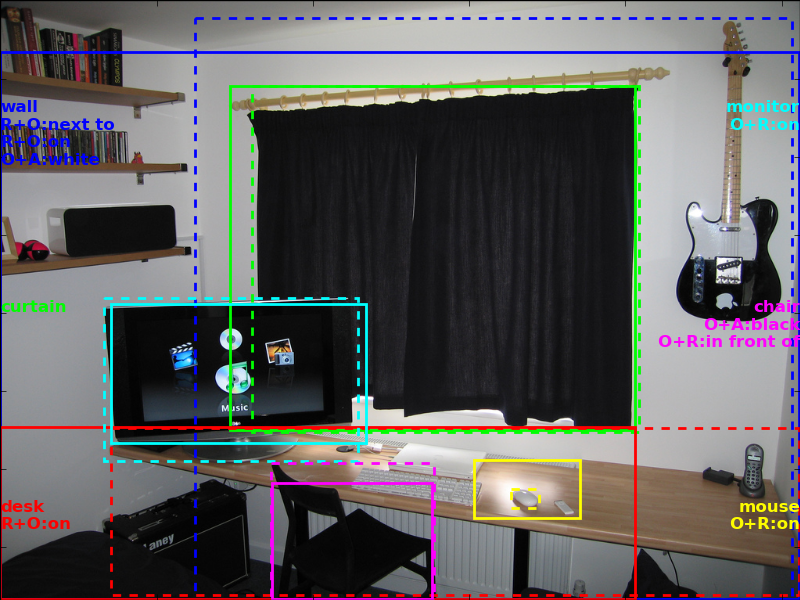
\includegraphics[width=2.7cm]{3_opt.png}
%    \vspace{0.0in}
    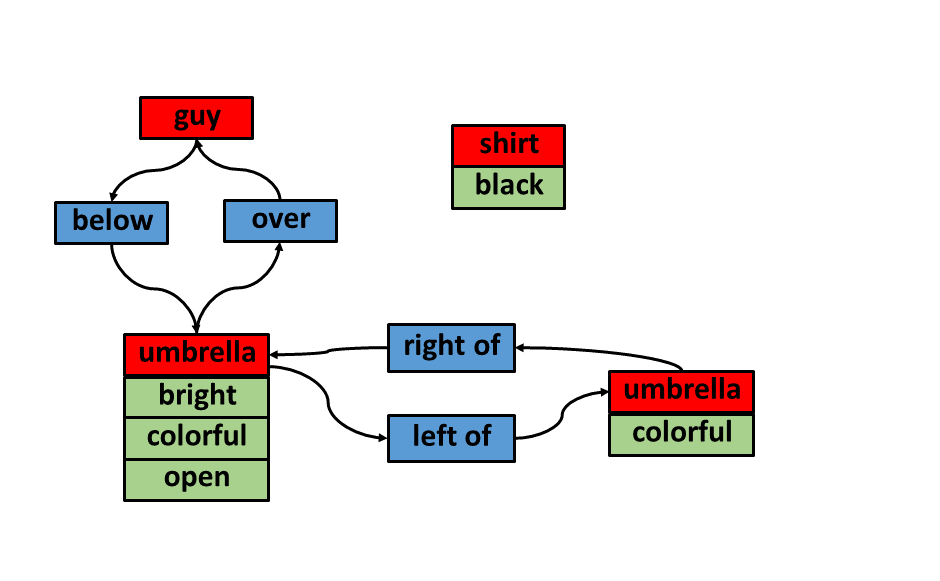
\includegraphics[width=2.7cm]{19_scene_graph.png}\hspace{0em}
    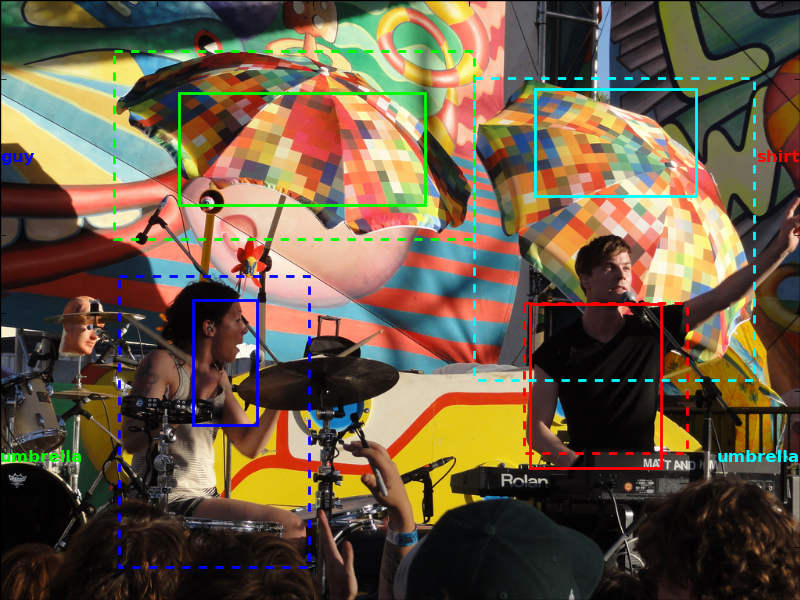
\includegraphics[width=2.7cm]{19_ind.png}\hspace{0em}
    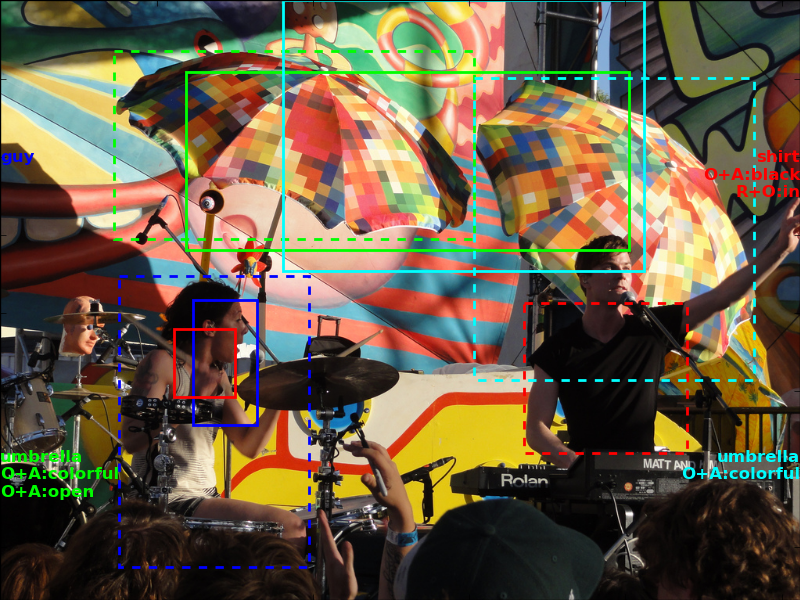
\includegraphics[width=2.7cm]{19_joint.png}\hspace{0em} 
    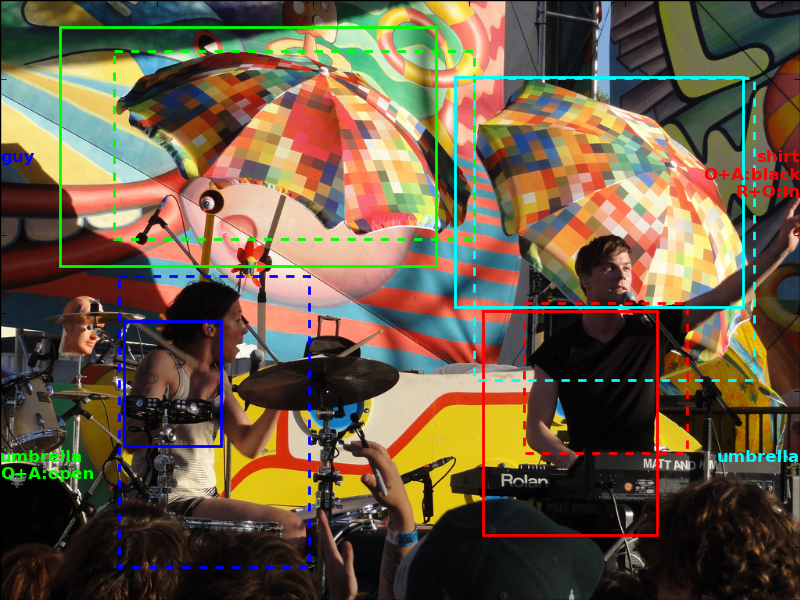
\includegraphics[width=2.7cm]{19_opt.png}
    \vspace{0.0in}
%    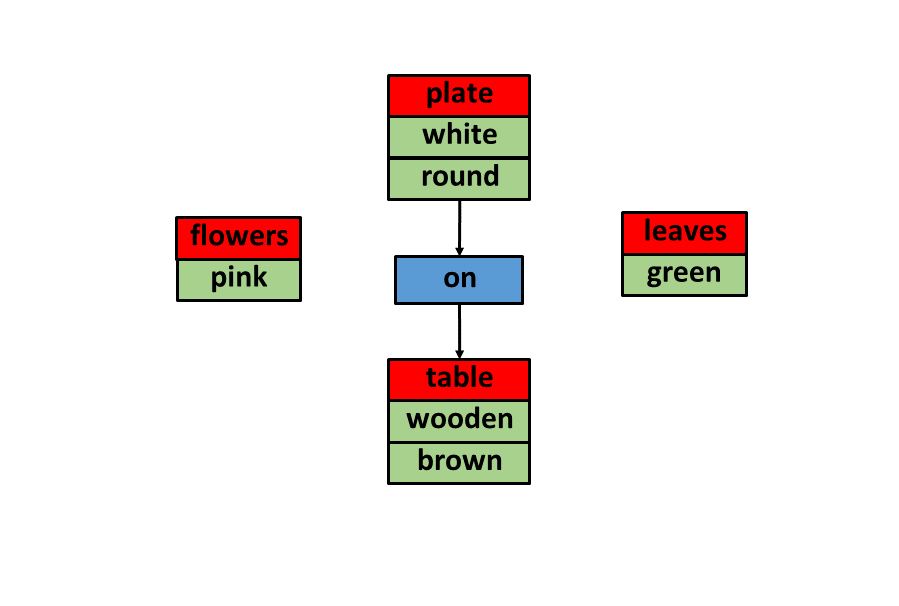
\includegraphics[width=2.7cm]{27_scene_graph.png}\hspace{0em}
%    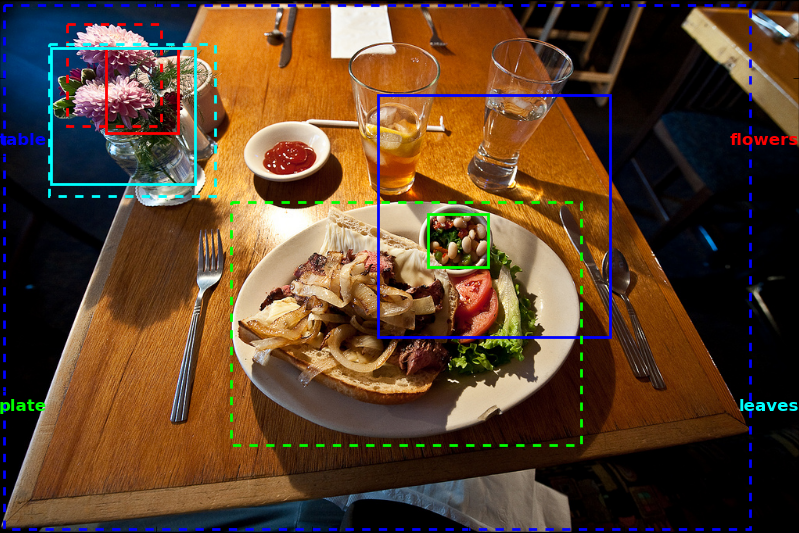
\includegraphics[width=2.7cm]{27_ind.png}\hspace{0em}
%    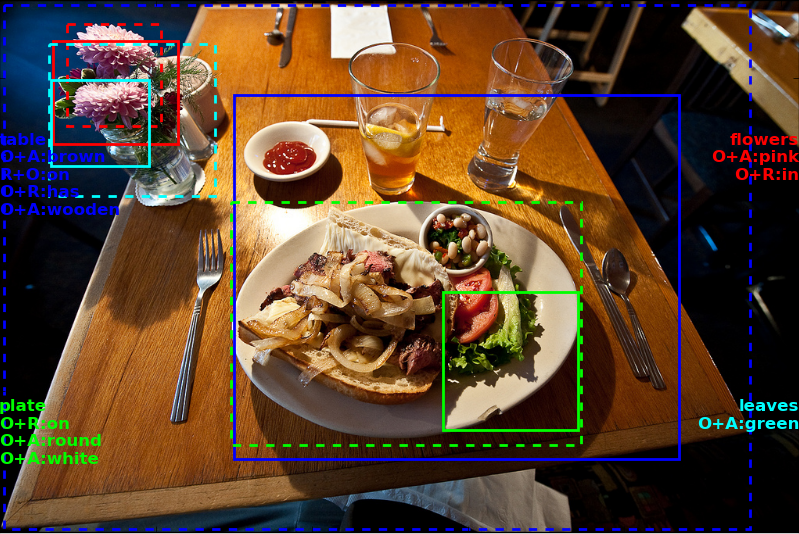
\includegraphics[width=2.7cm]{27_joint.png}\hspace{0em} 
%    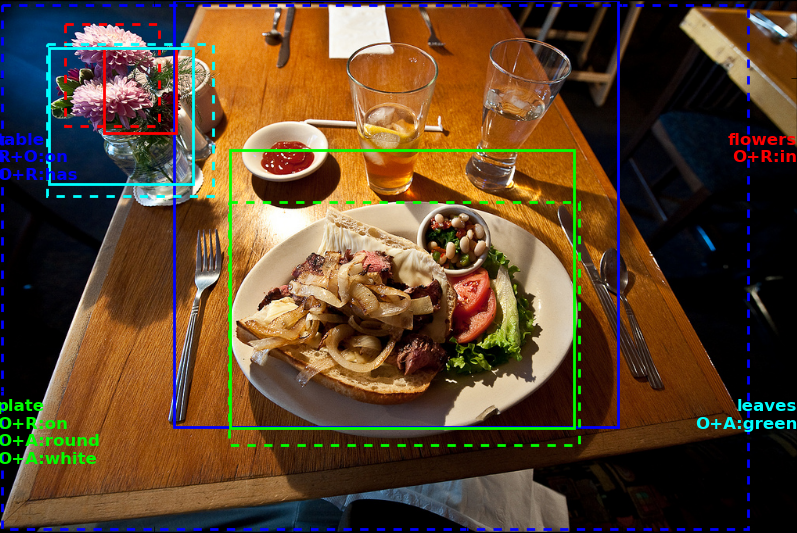
\includegraphics[width=2.7cm]{27_opt.png}
%    \vspace{0.0in}
    \centering
    \subcaptionbox{Scene graph}{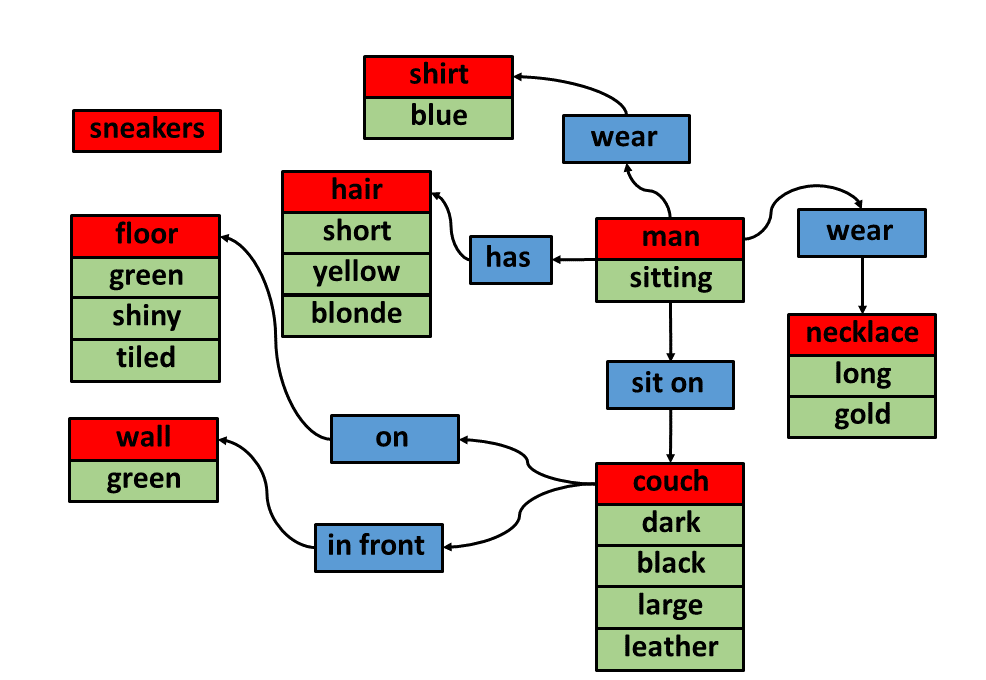
\includegraphics[width=2.7cm]{52_scene_graph.png}}\hspace{0em}
    \subcaptionbox{Independent}{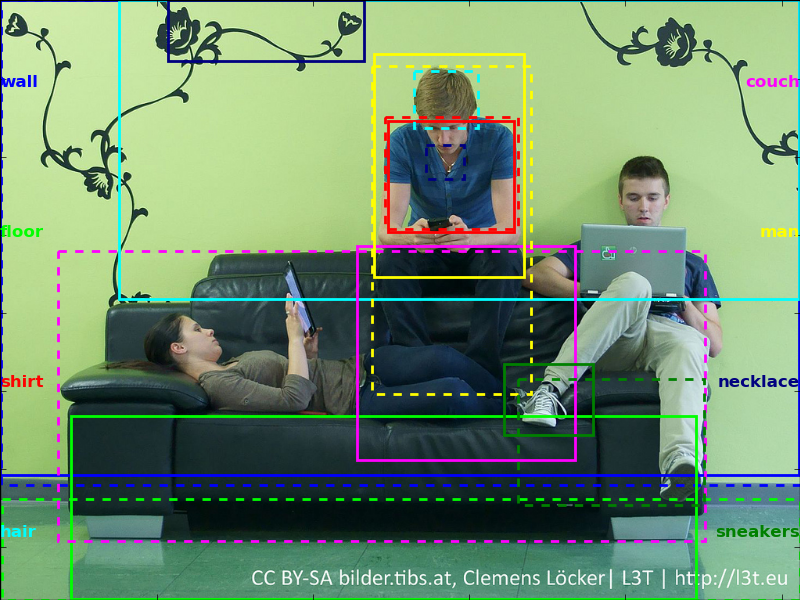
\includegraphics[width=2.7cm]{52_ind.png}}\hspace{0em}
    \subcaptionbox{Joint}{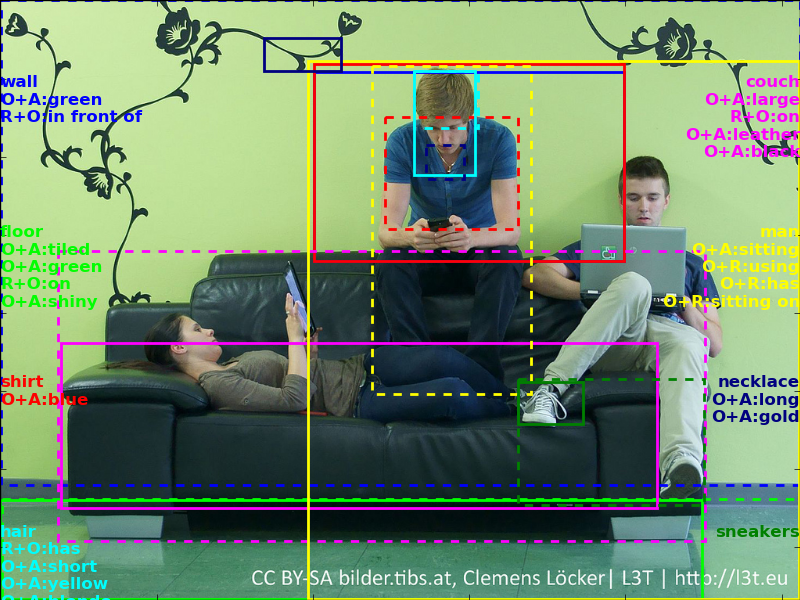
\includegraphics[width=2.7cm]{52_joint.png}}\hspace{0em}
    \subcaptionbox{Our method}{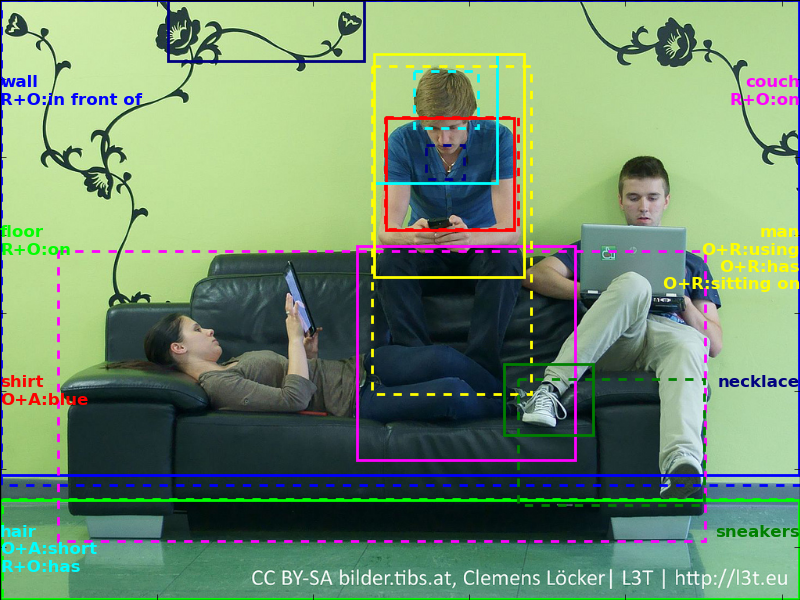
\includegraphics[width=2.7cm]{52_opt.png}}

    \caption{{\bf Qualitative results for SceneGraph retrieval:} Illustrated is (a) partial query scene graph, and grounding of objects obtained using (b) independent, (c) joint and (d) predicted, using our regression method, detector strategy. Dashed boxes are ground truth annotations. At the side of each image are shown the joint composites used for each object. independent is using none, joint is using all, and our method is selecting part of them.}%
    \label{fig:scene_graph_retrieval}%
\vspace*{-\baselineskip}
\vspace*{-\baselineskip}
% \vspace{-0.1in}    
\end{figure}

\end{document}